\subsection*{A1. Stock Return Data}\label{sec:appendixa1}

\begin{table}[!ht]
  \centering
  \caption{\textbf{Summary Statistics of Stock Returns}}
  \begin{tabular}{lcccc}
  \hline
      ~ & CAPM ab\_return & FF3 ab\_return & FF5 ab\_return & Excess return \\ \hline
      Count & 1397937 & 1397937 & 1397937 & 1397937 \\ 
      Mean & 0.001 & 0.000 & 0.001 & 0.009 \\ 
      Std & 0.163 & 0.165 & 0.173 & 0.170 \\ 
      Min & -2.306 & -2.748 & -4.295 & -0.985 \\ 
      25\% & -0.070 & -0.072 & -0.074 & -0.067 \\ 
      50\% & -0.007 & -0.008 & -0.007 & -0.002 \\ 
      75\% & 0.057 & 0.058 & 0.062 & 0.069 \\ 
      Max & 18.920 & 18.928 & 19.043 & 18.998 \\ \hline
  \end{tabular}
  \label{table: Summary statistic of return}
\end{table}

\begin{figure}[H]
  \centering
  \caption{\textbf{Correlation Between Stock Returns}}
  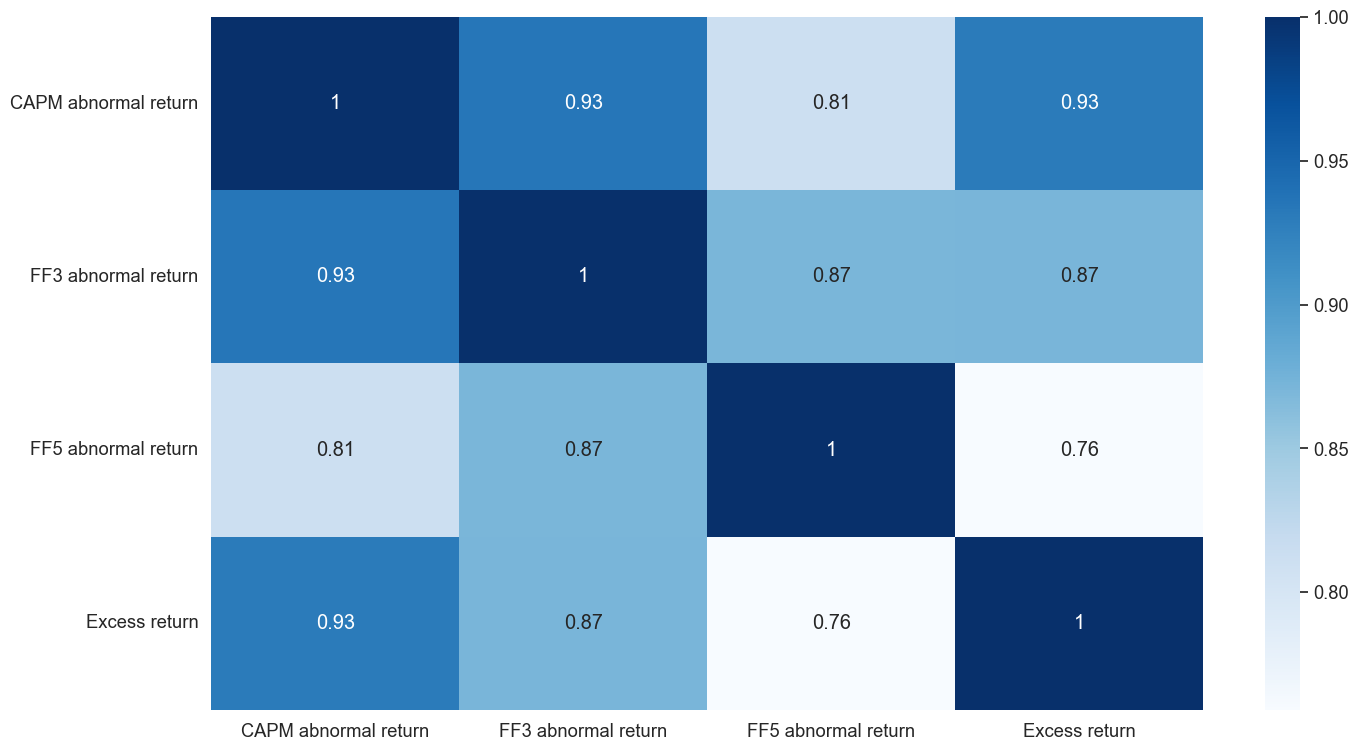
\includegraphics[width=.8\textwidth]{images/abnormal_excess_corr.png}
  \label{fig: abnormal_excess_corr}
  \caption*{\footnotesize{This figure plots the heatmap of correlations among each different measurements of stock returns.}}
\end{figure} 

\subsection*{A2. Macroeconomic Data}\label{sec:appendixa2}
The CFNAI index is composed of 85 economic indicators, it also includes indices covering four broad categories:
\begin{itemize}
  \item Production and income: measures of output, income, and sales, including indicators such as industrial production, personal income, and manufacturing and trade sales.

  \item Employment, unemployment, and hours: measures of labor market activity, including indicators such as nonfarm payrolls, unemployment rate, and average weekly hours.
  
  \item Personal consumption and housing: measures of consumer spending and housing activity, including indicators such as retail sales, housing starts, and new home sales.
  
  \item Sales, orders, and inventories: measures of business activity, including indicators such as durable goods orders, wholesale trade inventories, and new orders for nondefense capital goods.
\end{itemize}

\begin{figure}[H]
  \centering
  \caption{\textbf{Subsectional Macroeconomic indices}}
  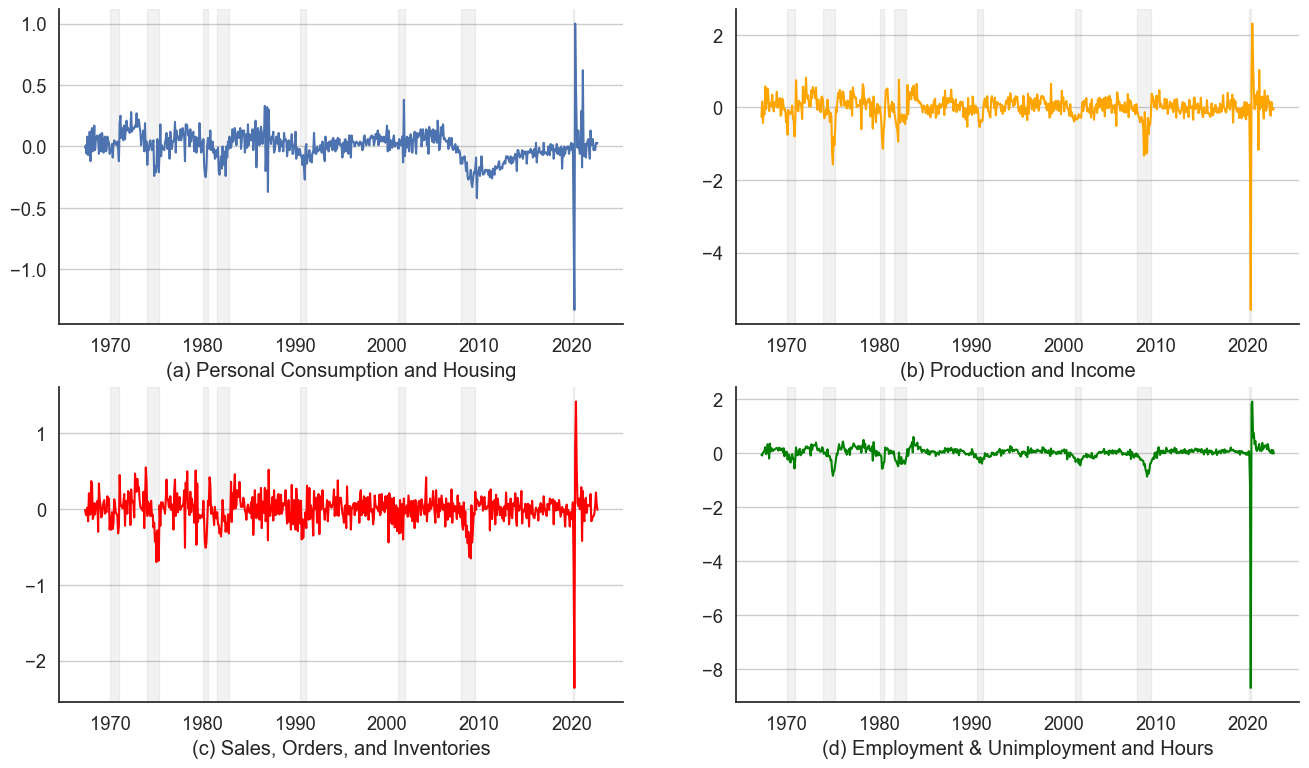
\includegraphics[width=.8\textwidth]{images/cfnai_four_components.png}
  \label{fig: Subsectional Macroeconomic index}
  \caption*{\footnotesize{This figure plots the subsectional macroeconomic indices from the CFNAI index dataset together with the NBER suggested recession periods with shaded bars.}}
\end{figure} 

The investor's sentiment data is composed by five indicators including:

\begin{itemize}
  \item Dividend premium: measures the difference between the value-weighted dividend yield of stocks and the yield on long-term government bonds.
  \item First day return on IPO: measures the percentage change in stock price from the offer price to the first day of trading.
  \item Closed-end fund discount: measures the difference between the market price and the net asset value of a closed-end fund.
  \item IPO valume: measures the number of new issues in a month.
  \item Equity share in new issues: measures the percentage of new issues in which the issuing company retains less than half of the outstanding equity.
\end{itemize}

\begin{figure}[H]
  \centering
  \caption{\textbf{5 Components for Composing Sentiment Index}}
  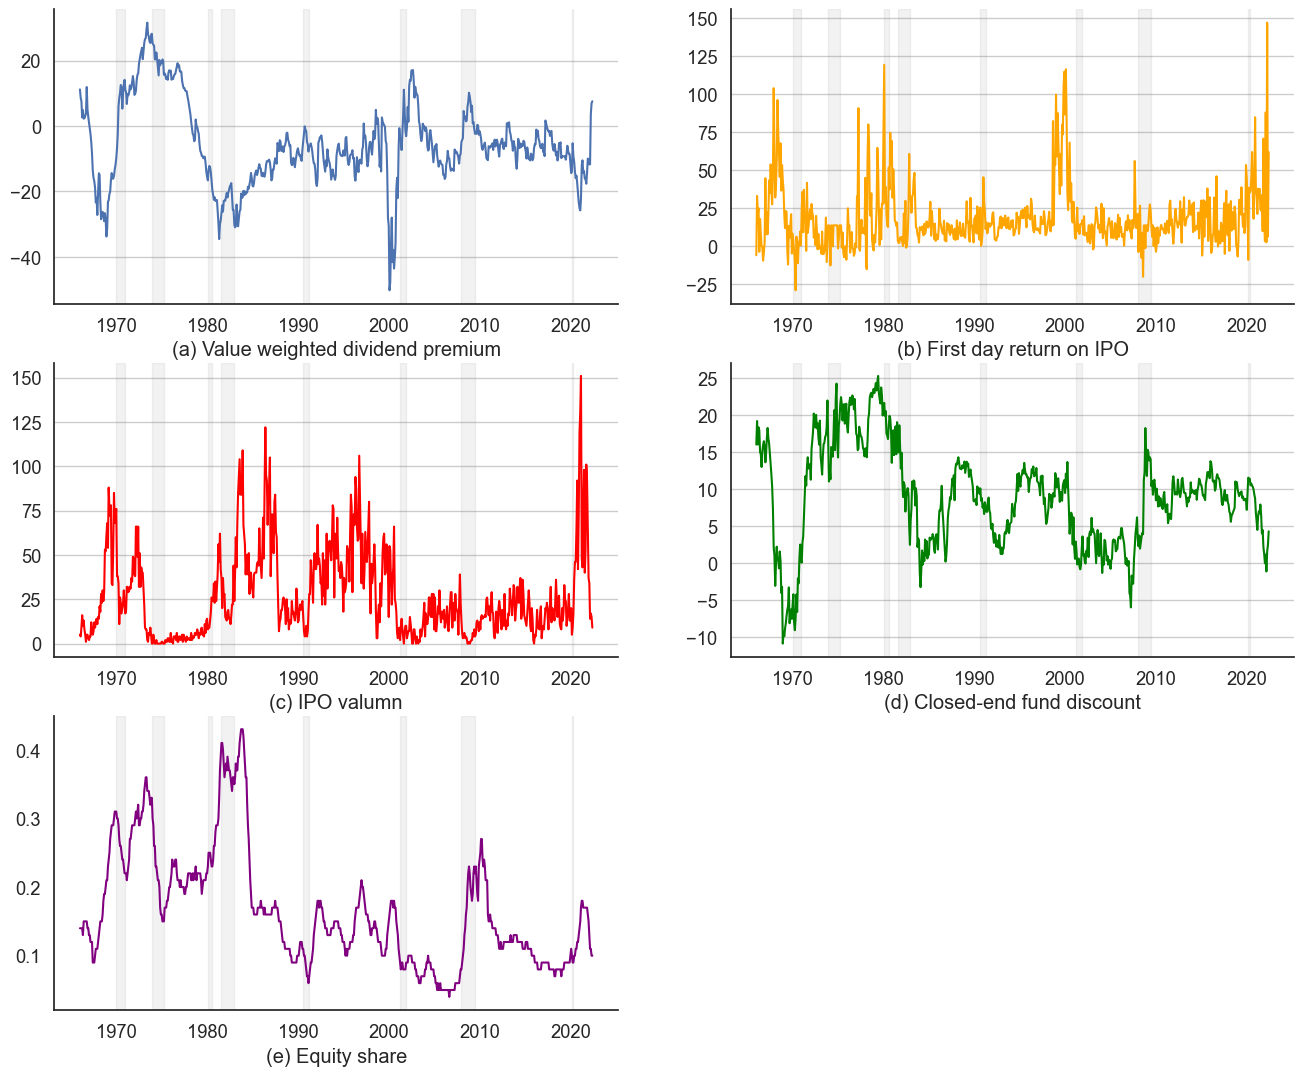
\includegraphics[width=.8\textwidth]{images/sent_5_components.png}
  \label{fig: 5 components for sentiment}
  \caption*{\footnotesize{This figure plots the 5 components for composing investor's sentiment index together with the NBER suggested recession periods with shaded bars.}}
\end{figure} 